%\documentclass{standalone}
%\usepackage{tikz}
%\usetikzlibrary{patterns,plotmarks}
%\begin{document}
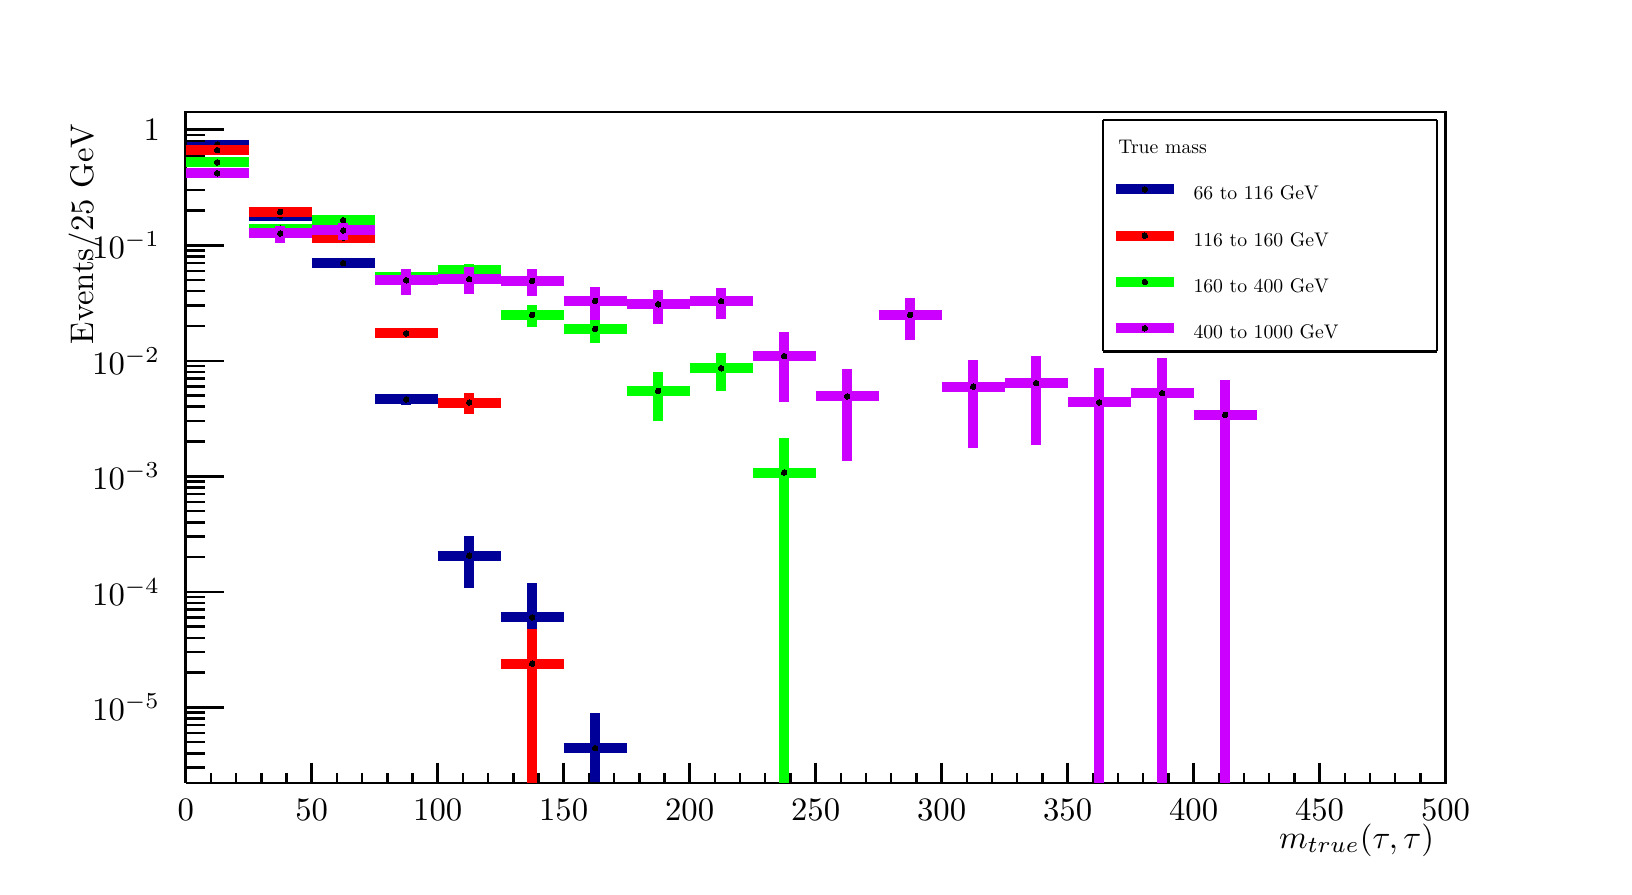
\begin{tikzpicture}
\def\CheckTikzLibraryLoaded#1{ \ifcsname tikz@library@#1@loaded\endcsname \else \PackageWarning{tikz}{usetikzlibrary{#1} is missing in the preamble.} \fi }
\CheckTikzLibraryLoaded{patterns}
\CheckTikzLibraryLoaded{plotmarks}
\pgfdeclareplotmark{cross} {
\pgfpathmoveto{\pgfpoint{-0.3\pgfplotmarksize}{\pgfplotmarksize}}
\pgfpathlineto{\pgfpoint{+0.3\pgfplotmarksize}{\pgfplotmarksize}}
\pgfpathlineto{\pgfpoint{+0.3\pgfplotmarksize}{0.3\pgfplotmarksize}}
\pgfpathlineto{\pgfpoint{+1\pgfplotmarksize}{0.3\pgfplotmarksize}}
\pgfpathlineto{\pgfpoint{+1\pgfplotmarksize}{-0.3\pgfplotmarksize}}
\pgfpathlineto{\pgfpoint{+0.3\pgfplotmarksize}{-0.3\pgfplotmarksize}}
\pgfpathlineto{\pgfpoint{+0.3\pgfplotmarksize}{-1.\pgfplotmarksize}}
\pgfpathlineto{\pgfpoint{-0.3\pgfplotmarksize}{-1.\pgfplotmarksize}}
\pgfpathlineto{\pgfpoint{-0.3\pgfplotmarksize}{-0.3\pgfplotmarksize}}
\pgfpathlineto{\pgfpoint{-1.\pgfplotmarksize}{-0.3\pgfplotmarksize}}
\pgfpathlineto{\pgfpoint{-1.\pgfplotmarksize}{0.3\pgfplotmarksize}}
\pgfpathlineto{\pgfpoint{-0.3\pgfplotmarksize}{0.3\pgfplotmarksize}}
\pgfpathclose
\pgfusepathqstroke
}
\pgfdeclareplotmark{cross*} {
\pgfpathmoveto{\pgfpoint{-0.3\pgfplotmarksize}{\pgfplotmarksize}}
\pgfpathlineto{\pgfpoint{+0.3\pgfplotmarksize}{\pgfplotmarksize}}
\pgfpathlineto{\pgfpoint{+0.3\pgfplotmarksize}{0.3\pgfplotmarksize}}
\pgfpathlineto{\pgfpoint{+1\pgfplotmarksize}{0.3\pgfplotmarksize}}
\pgfpathlineto{\pgfpoint{+1\pgfplotmarksize}{-0.3\pgfplotmarksize}}
\pgfpathlineto{\pgfpoint{+0.3\pgfplotmarksize}{-0.3\pgfplotmarksize}}
\pgfpathlineto{\pgfpoint{+0.3\pgfplotmarksize}{-1.\pgfplotmarksize}}
\pgfpathlineto{\pgfpoint{-0.3\pgfplotmarksize}{-1.\pgfplotmarksize}}
\pgfpathlineto{\pgfpoint{-0.3\pgfplotmarksize}{-0.3\pgfplotmarksize}}
\pgfpathlineto{\pgfpoint{-1.\pgfplotmarksize}{-0.3\pgfplotmarksize}}
\pgfpathlineto{\pgfpoint{-1.\pgfplotmarksize}{0.3\pgfplotmarksize}}
\pgfpathlineto{\pgfpoint{-0.3\pgfplotmarksize}{0.3\pgfplotmarksize}}
\pgfpathclose
\pgfusepathqfillstroke
}
\pgfdeclareplotmark{newstar} {
\pgfpathmoveto{\pgfqpoint{0pt}{\pgfplotmarksize}}
\pgfpathlineto{\pgfqpointpolar{44}{0.5\pgfplotmarksize}}
\pgfpathlineto{\pgfqpointpolar{18}{\pgfplotmarksize}}
\pgfpathlineto{\pgfqpointpolar{-20}{0.5\pgfplotmarksize}}
\pgfpathlineto{\pgfqpointpolar{-54}{\pgfplotmarksize}}
\pgfpathlineto{\pgfqpointpolar{-90}{0.5\pgfplotmarksize}}
\pgfpathlineto{\pgfqpointpolar{234}{\pgfplotmarksize}}
\pgfpathlineto{\pgfqpointpolar{198}{0.5\pgfplotmarksize}}
\pgfpathlineto{\pgfqpointpolar{162}{\pgfplotmarksize}}
\pgfpathlineto{\pgfqpointpolar{134}{0.5\pgfplotmarksize}}
\pgfpathclose
\pgfusepathqstroke
}
\pgfdeclareplotmark{newstar*} {
\pgfpathmoveto{\pgfqpoint{0pt}{\pgfplotmarksize}}
\pgfpathlineto{\pgfqpointpolar{44}{0.5\pgfplotmarksize}}
\pgfpathlineto{\pgfqpointpolar{18}{\pgfplotmarksize}}
\pgfpathlineto{\pgfqpointpolar{-20}{0.5\pgfplotmarksize}}
\pgfpathlineto{\pgfqpointpolar{-54}{\pgfplotmarksize}}
\pgfpathlineto{\pgfqpointpolar{-90}{0.5\pgfplotmarksize}}
\pgfpathlineto{\pgfqpointpolar{234}{\pgfplotmarksize}}
\pgfpathlineto{\pgfqpointpolar{198}{0.5\pgfplotmarksize}}
\pgfpathlineto{\pgfqpointpolar{162}{\pgfplotmarksize}}
\pgfpathlineto{\pgfqpointpolar{134}{0.5\pgfplotmarksize}}
\pgfpathclose
\pgfusepathqfillstroke
}
\definecolor{c}{rgb}{1,1,1};
\draw [color=c, fill=c] (0,0) rectangle (20,10.6489);
\draw [color=c, fill=c] (2,1.06489) rectangle (18,9.58405);
\definecolor{c}{rgb}{0,0,0};
\draw [c,line width=0.9] (2,1.06489) -- (2,9.58405) -- (18,9.58405) -- (18,1.06489) -- (2,1.06489);
\definecolor{c}{rgb}{1,1,1};
\draw [color=c, fill=c] (2,1.06489) rectangle (18,9.58405);
\definecolor{c}{rgb}{0,0,0};
\draw [c,line width=0.9] (2,1.06489) -- (2,9.58405) -- (18,9.58405) -- (18,1.06489) -- (2,1.06489);
\definecolor{c}{rgb}{0,0,0.6};
\draw [c,line width=3.6] (2.4,9.16591) -- (2.4,9.17142);
\draw [c,line width=3.6] (2.4,9.17142) -- (2.4,9.17688);
\draw [c,line width=3.6] (2,9.17142) -- (2.4,9.17142);
\draw [c,line width=3.6] (2.4,9.17142) -- (2.8,9.17142);
\definecolor{c}{rgb}{0,0,0};
\foreach \P in {(2.4,9.17142)}{\draw[mark options={color=c,fill=c},mark size=2.402402pt, line width=0.000000pt, mark=*,mark size=1pt] plot coordinates {\P};}
\definecolor{c}{rgb}{0,0,0.6};
\draw [c,line width=3.6] (3.2,8.25758) -- (3.2,8.26879);
\draw [c,line width=3.6] (3.2,8.26879) -- (3.2,8.27981);
\draw [c,line width=3.6] (2.8,8.26879) -- (3.2,8.26879);
\draw [c,line width=3.6] (3.2,8.26879) -- (3.6,8.26879);
\definecolor{c}{rgb}{0,0,0};
\foreach \P in {(3.2,8.26879)}{\draw[mark options={color=c,fill=c},mark size=2.402402pt, line width=0.000000pt, mark=*,mark size=1pt] plot coordinates {\P};}
\definecolor{c}{rgb}{0,0,0.6};
\draw [c,line width=3.6] (4,7.64893) -- (4,7.66691);
\draw [c,line width=3.6] (4,7.66691) -- (4,7.6844);
\draw [c,line width=3.6] (3.6,7.66691) -- (4,7.66691);
\draw [c,line width=3.6] (4,7.66691) -- (4.4,7.66691);
\definecolor{c}{rgb}{0,0,0};
\foreach \P in {(4,7.66691)}{\draw[mark options={color=c,fill=c},mark size=2.402402pt, line width=0.000000pt, mark=*,mark size=1pt] plot coordinates {\P};}
\definecolor{c}{rgb}{0,0,0.6};
\draw [c,line width=3.6] (4.8,5.86177) -- (4.8,5.93464);
\draw [c,line width=3.6] (4.8,5.93464) -- (4.8,6.00002);
\draw [c,line width=3.6] (4.4,5.93464) -- (4.8,5.93464);
\draw [c,line width=3.6] (4.8,5.93464) -- (5.2,5.93464);
\definecolor{c}{rgb}{0,0,0};
\foreach \P in {(4.8,5.93464)}{\draw[mark options={color=c,fill=c},mark size=2.402402pt, line width=0.000000pt, mark=*,mark size=1pt] plot coordinates {\P};}
\definecolor{c}{rgb}{0,0,0.6};
\draw [c,line width=3.6] (5.6,3.54127) -- (5.6,3.9498);
\draw [c,line width=3.6] (5.6,3.9498) -- (5.6,4.19671);
\draw [c,line width=3.6] (5.2,3.9498) -- (5.6,3.9498);
\draw [c,line width=3.6] (5.6,3.9498) -- (6,3.9498);
\definecolor{c}{rgb}{0,0,0};
\foreach \P in {(5.6,3.9498)}{\draw[mark options={color=c,fill=c},mark size=2.402402pt, line width=0.000000pt, mark=*,mark size=1pt] plot coordinates {\P};}
\definecolor{c}{rgb}{0,0,0.6};
\draw [c,line width=3.6] (6.4,1.06489) -- (6.4,3.16624);
\draw [c,line width=3.6] (6.4,3.16624) -- (6.4,3.60786);
\draw [c,line width=3.6] (6,3.16624) -- (6.4,3.16624);
\draw [c,line width=3.6] (6.4,3.16624) -- (6.8,3.16624);
\definecolor{c}{rgb}{0,0,0};
\foreach \P in {(6.4,3.16624)}{\draw[mark options={color=c,fill=c},mark size=2.402402pt, line width=0.000000pt, mark=*,mark size=1pt] plot coordinates {\P};}
\definecolor{c}{rgb}{0,0,0.6};
\draw [c,line width=3.6] (7.2,1.06489) -- (7.2,1.50652);
\draw [c,line width=3.6] (7.2,1.50652) -- (7.2,1.94814);
\draw [c,line width=3.6] (6.8,1.50652) -- (7.2,1.50652);
\draw [c,line width=3.6] (7.2,1.50652) -- (7.6,1.50652);
\definecolor{c}{rgb}{0,0,0};
\foreach \P in {(7.2,1.50652)}{\draw[mark options={color=c,fill=c},mark size=2.402402pt, line width=0.000000pt, mark=*,mark size=1pt] plot coordinates {\P};}
\draw [c,line width=0.9] (2,1.06489) -- (18,1.06489);
\draw [c,line width=0.9] (2,1.32047) -- (2,1.06489);
\draw [c,line width=0.9] (2.32,1.19268) -- (2.32,1.06489);
\draw [c,line width=0.9] (2.64,1.19268) -- (2.64,1.06489);
\draw [c,line width=0.9] (2.96,1.19268) -- (2.96,1.06489);
\draw [c,line width=0.9] (3.28,1.19268) -- (3.28,1.06489);
\draw [c,line width=0.9] (3.6,1.32047) -- (3.6,1.06489);
\draw [c,line width=0.9] (3.92,1.19268) -- (3.92,1.06489);
\draw [c,line width=0.9] (4.24,1.19268) -- (4.24,1.06489);
\draw [c,line width=0.9] (4.56,1.19268) -- (4.56,1.06489);
\draw [c,line width=0.9] (4.88,1.19268) -- (4.88,1.06489);
\draw [c,line width=0.9] (5.2,1.32047) -- (5.2,1.06489);
\draw [c,line width=0.9] (5.52,1.19268) -- (5.52,1.06489);
\draw [c,line width=0.9] (5.84,1.19268) -- (5.84,1.06489);
\draw [c,line width=0.9] (6.16,1.19268) -- (6.16,1.06489);
\draw [c,line width=0.9] (6.48,1.19268) -- (6.48,1.06489);
\draw [c,line width=0.9] (6.8,1.32047) -- (6.8,1.06489);
\draw [c,line width=0.9] (7.12,1.19268) -- (7.12,1.06489);
\draw [c,line width=0.9] (7.44,1.19268) -- (7.44,1.06489);
\draw [c,line width=0.9] (7.76,1.19268) -- (7.76,1.06489);
\draw [c,line width=0.9] (8.08,1.19268) -- (8.08,1.06489);
\draw [c,line width=0.9] (8.4,1.32047) -- (8.4,1.06489);
\draw [c,line width=0.9] (8.72,1.19268) -- (8.72,1.06489);
\draw [c,line width=0.9] (9.04,1.19268) -- (9.04,1.06489);
\draw [c,line width=0.9] (9.36,1.19268) -- (9.36,1.06489);
\draw [c,line width=0.9] (9.68,1.19268) -- (9.68,1.06489);
\draw [c,line width=0.9] (10,1.32047) -- (10,1.06489);
\draw [c,line width=0.9] (10.32,1.19268) -- (10.32,1.06489);
\draw [c,line width=0.9] (10.64,1.19268) -- (10.64,1.06489);
\draw [c,line width=0.9] (10.96,1.19268) -- (10.96,1.06489);
\draw [c,line width=0.9] (11.28,1.19268) -- (11.28,1.06489);
\draw [c,line width=0.9] (11.6,1.32047) -- (11.6,1.06489);
\draw [c,line width=0.9] (11.92,1.19268) -- (11.92,1.06489);
\draw [c,line width=0.9] (12.24,1.19268) -- (12.24,1.06489);
\draw [c,line width=0.9] (12.56,1.19268) -- (12.56,1.06489);
\draw [c,line width=0.9] (12.88,1.19268) -- (12.88,1.06489);
\draw [c,line width=0.9] (13.2,1.32047) -- (13.2,1.06489);
\draw [c,line width=0.9] (13.52,1.19268) -- (13.52,1.06489);
\draw [c,line width=0.9] (13.84,1.19268) -- (13.84,1.06489);
\draw [c,line width=0.9] (14.16,1.19268) -- (14.16,1.06489);
\draw [c,line width=0.9] (14.48,1.19268) -- (14.48,1.06489);
\draw [c,line width=0.9] (14.8,1.32047) -- (14.8,1.06489);
\draw [c,line width=0.9] (15.12,1.19268) -- (15.12,1.06489);
\draw [c,line width=0.9] (15.44,1.19268) -- (15.44,1.06489);
\draw [c,line width=0.9] (15.76,1.19268) -- (15.76,1.06489);
\draw [c,line width=0.9] (16.08,1.19268) -- (16.08,1.06489);
\draw [c,line width=0.9] (16.4,1.32047) -- (16.4,1.06489);
\draw [c,line width=0.9] (16.72,1.19268) -- (16.72,1.06489);
\draw [c,line width=0.9] (17.04,1.19268) -- (17.04,1.06489);
\draw [c,line width=0.9] (17.36,1.19268) -- (17.36,1.06489);
\draw [c,line width=0.9] (17.68,1.19268) -- (17.68,1.06489);
\draw [c,line width=0.9] (18,1.32047) -- (18,1.06489);
\draw [anchor=base] (2,0.585692) node[scale=1.18081, color=c, rotate=0]{0};
\draw [anchor=base] (3.6,0.585692) node[scale=1.18081, color=c, rotate=0]{50};
\draw [anchor=base] (5.2,0.585692) node[scale=1.18081, color=c, rotate=0]{100};
\draw [anchor=base] (6.8,0.585692) node[scale=1.18081, color=c, rotate=0]{150};
\draw [anchor=base] (8.4,0.585692) node[scale=1.18081, color=c, rotate=0]{200};
\draw [anchor=base] (10,0.585692) node[scale=1.18081, color=c, rotate=0]{250};
\draw [anchor=base] (11.6,0.585692) node[scale=1.18081, color=c, rotate=0]{300};
\draw [anchor=base] (13.2,0.585692) node[scale=1.18081, color=c, rotate=0]{350};
\draw [anchor=base] (14.8,0.585692) node[scale=1.18081, color=c, rotate=0]{400};
\draw [anchor=base] (16.4,0.585692) node[scale=1.18081, color=c, rotate=0]{450};
\draw [anchor=base] (18,0.585692) node[scale=1.18081, color=c, rotate=0]{500};
\draw [anchor= east] (18,0.340766) node[scale=1.18081, color=c, rotate=0]{$m_{true}(\tau,\tau)$};
\draw [c,line width=0.9] (2,1.06489) -- (2,9.58405);
\draw [c,line width=0.9] (2.24,1.25725) -- (2,1.25725);
\draw [c,line width=0.9] (2.24,1.44054) -- (2,1.44054);
\draw [c,line width=0.9] (2.24,1.58271) -- (2,1.58271);
\draw [c,line width=0.9] (2.24,1.69887) -- (2,1.69887);
\draw [c,line width=0.9] (2.24,1.79709) -- (2,1.79709);
\draw [c,line width=0.9] (2.24,1.88216) -- (2,1.88216);
\draw [c,line width=0.9] (2.24,1.9572) -- (2,1.9572);
\draw [c,line width=0.9] (2.48,2.02433) -- (2,2.02433);
\draw [anchor= east] (1.82,2.02433) node[scale=1.18081, color=c, rotate=0]{$10^{-5}$};
\draw [c,line width=0.9] (2.24,2.46595) -- (2,2.46595);
\draw [c,line width=0.9] (2.24,2.72428) -- (2,2.72428);
\draw [c,line width=0.9] (2.24,2.90757) -- (2,2.90757);
\draw [c,line width=0.9] (2.24,3.04974) -- (2,3.04974);
\draw [c,line width=0.9] (2.24,3.1659) -- (2,3.1659);
\draw [c,line width=0.9] (2.24,3.26412) -- (2,3.26412);
\draw [c,line width=0.9] (2.24,3.34919) -- (2,3.34919);
\draw [c,line width=0.9] (2.24,3.42424) -- (2,3.42424);
\draw [c,line width=0.9] (2.48,3.49136) -- (2,3.49136);
\draw [anchor= east] (1.82,3.49136) node[scale=1.18081, color=c, rotate=0]{$10^{-4}$};
\draw [c,line width=0.9] (2.24,3.93298) -- (2,3.93298);
\draw [c,line width=0.9] (2.24,4.19132) -- (2,4.19132);
\draw [c,line width=0.9] (2.24,4.3746) -- (2,4.3746);
\draw [c,line width=0.9] (2.24,4.51677) -- (2,4.51677);
\draw [c,line width=0.9] (2.24,4.63294) -- (2,4.63294);
\draw [c,line width=0.9] (2.24,4.73115) -- (2,4.73115);
\draw [c,line width=0.9] (2.24,4.81623) -- (2,4.81623);
\draw [c,line width=0.9] (2.24,4.89127) -- (2,4.89127);
\draw [c,line width=0.9] (2.48,4.9584) -- (2,4.9584);
\draw [anchor= east] (1.82,4.9584) node[scale=1.18081, color=c, rotate=0]{$10^{-3}$};
\draw [c,line width=0.9] (2.24,5.40002) -- (2,5.40002);
\draw [c,line width=0.9] (2.24,5.65835) -- (2,5.65835);
\draw [c,line width=0.9] (2.24,5.84164) -- (2,5.84164);
\draw [c,line width=0.9] (2.24,5.98381) -- (2,5.98381);
\draw [c,line width=0.9] (2.24,6.09997) -- (2,6.09997);
\draw [c,line width=0.9] (2.24,6.19818) -- (2,6.19818);
\draw [c,line width=0.9] (2.24,6.28326) -- (2,6.28326);
\draw [c,line width=0.9] (2.24,6.3583) -- (2,6.3583);
\draw [c,line width=0.9] (2.48,6.42543) -- (2,6.42543);
\draw [anchor= east] (1.82,6.42543) node[scale=1.18081, color=c, rotate=0]{$10^{-2}$};
\draw [c,line width=0.9] (2.24,6.86705) -- (2,6.86705);
\draw [c,line width=0.9] (2.24,7.12538) -- (2,7.12538);
\draw [c,line width=0.9] (2.24,7.30867) -- (2,7.30867);
\draw [c,line width=0.9] (2.24,7.45084) -- (2,7.45084);
\draw [c,line width=0.9] (2.24,7.567) -- (2,7.567);
\draw [c,line width=0.9] (2.24,7.66521) -- (2,7.66521);
\draw [c,line width=0.9] (2.24,7.75029) -- (2,7.75029);
\draw [c,line width=0.9] (2.24,7.82533) -- (2,7.82533);
\draw [c,line width=0.9] (2.48,7.89246) -- (2,7.89246);
\draw [anchor= east] (1.82,7.89246) node[scale=1.18081, color=c, rotate=0]{$10^{-1}$};
\draw [c,line width=0.9] (2.24,8.33408) -- (2,8.33408);
\draw [c,line width=0.9] (2.24,8.59241) -- (2,8.59241);
\draw [c,line width=0.9] (2.24,8.7757) -- (2,8.7757);
\draw [c,line width=0.9] (2.24,8.91787) -- (2,8.91787);
\draw [c,line width=0.9] (2.24,9.03403) -- (2,9.03403);
\draw [c,line width=0.9] (2.24,9.13224) -- (2,9.13224);
\draw [c,line width=0.9] (2.24,9.21732) -- (2,9.21732);
\draw [c,line width=0.9] (2.24,9.29236) -- (2,9.29236);
\draw [c,line width=0.9] (2.48,9.35949) -- (2,9.35949);
\draw [anchor= east] (1.82,9.35949) node[scale=1.18081, color=c, rotate=0]{1};
\draw [anchor= east] (0.72,9.58405) node[scale=1.18081, color=c, rotate=90]{Events/25 GeV};
\definecolor{c}{rgb}{1,0,0};
\draw [c,line width=3.6] (2.4,9.09536) -- (2.4,9.10144);
\draw [c,line width=3.6] (2.4,9.10144) -- (2.4,9.10746);
\draw [c,line width=3.6] (2,9.10144) -- (2.4,9.10144);
\draw [c,line width=3.6] (2.4,9.10144) -- (2.8,9.10144);
\definecolor{c}{rgb}{0,0,0};
\foreach \P in {(2.4,9.10144)}{\draw[mark options={color=c,fill=c},mark size=2.402402pt, line width=0.000000pt, mark=*,mark size=1pt] plot coordinates {\P};}
\definecolor{c}{rgb}{1,0,0};
\draw [c,line width=3.6] (3.2,8.30587) -- (3.2,8.31756);
\draw [c,line width=3.6] (3.2,8.31756) -- (3.2,8.32905);
\draw [c,line width=3.6] (2.8,8.31756) -- (3.2,8.31756);
\draw [c,line width=3.6] (3.2,8.31756) -- (3.6,8.31756);
\definecolor{c}{rgb}{0,0,0};
\foreach \P in {(3.2,8.31756)}{\draw[mark options={color=c,fill=c},mark size=2.402402pt, line width=0.000000pt, mark=*,mark size=1pt] plot coordinates {\P};}
\definecolor{c}{rgb}{1,0,0};
\draw [c,line width=3.6] (4,7.97354) -- (4,7.98976);
\draw [c,line width=3.6] (4,7.98976) -- (4,8.00558);
\draw [c,line width=3.6] (3.6,7.98976) -- (4,7.98976);
\draw [c,line width=3.6] (4,7.98976) -- (4.4,7.98976);
\definecolor{c}{rgb}{0,0,0};
\foreach \P in {(4,7.98976)}{\draw[mark options={color=c,fill=c},mark size=2.402402pt, line width=0.000000pt, mark=*,mark size=1pt] plot coordinates {\P};}
\definecolor{c}{rgb}{1,0,0};
\draw [c,line width=3.6] (4.8,6.72651) -- (4.8,6.77391);
\draw [c,line width=3.6] (4.8,6.77391) -- (4.8,6.81804);
\draw [c,line width=3.6] (4.4,6.77391) -- (4.8,6.77391);
\draw [c,line width=3.6] (4.8,6.77391) -- (5.2,6.77391);
\definecolor{c}{rgb}{0,0,0};
\foreach \P in {(4.8,6.77391)}{\draw[mark options={color=c,fill=c},mark size=2.402402pt, line width=0.000000pt, mark=*,mark size=1pt] plot coordinates {\P};}
\definecolor{c}{rgb}{1,0,0};
\draw [c,line width=3.6] (5.6,5.75508) -- (5.6,5.89529);
\draw [c,line width=3.6] (5.6,5.89529) -- (5.6,6.01015);
\draw [c,line width=3.6] (5.2,5.89529) -- (5.6,5.89529);
\draw [c,line width=3.6] (5.6,5.89529) -- (6,5.89529);
\definecolor{c}{rgb}{0,0,0};
\foreach \P in {(5.6,5.89529)}{\draw[mark options={color=c,fill=c},mark size=2.402402pt, line width=0.000000pt, mark=*,mark size=1pt] plot coordinates {\P};}
\definecolor{c}{rgb}{1,0,0};
\draw [c,line width=3.6] (6.4,1.06489) -- (6.4,2.57928);
\draw [c,line width=3.6] (6.4,2.57928) -- (6.4,3.0209);
\draw [c,line width=3.6] (6,2.57928) -- (6.4,2.57928);
\draw [c,line width=3.6] (6.4,2.57928) -- (6.8,2.57928);
\definecolor{c}{rgb}{0,0,0};
\foreach \P in {(6.4,2.57928)}{\draw[mark options={color=c,fill=c},mark size=2.402402pt, line width=0.000000pt, mark=*,mark size=1pt] plot coordinates {\P};}
\definecolor{c}{rgb}{0,1,0};
\draw [c,line width=3.6] (2.4,8.91543) -- (2.4,8.94539);
\draw [c,line width=3.6] (2.4,8.94539) -- (2.4,8.97401);
\draw [c,line width=3.6] (2,8.94539) -- (2.4,8.94539);
\draw [c,line width=3.6] (2.4,8.94539) -- (2.8,8.94539);
\definecolor{c}{rgb}{0,0,0};
\foreach \P in {(2.4,8.94539)}{\draw[mark options={color=c,fill=c},mark size=2.402402pt, line width=0.000000pt, mark=*,mark size=1pt] plot coordinates {\P};}
\definecolor{c}{rgb}{0,1,0};
\draw [c,line width=3.6] (3.2,8.04737) -- (3.2,8.10497);
\draw [c,line width=3.6] (3.2,8.10497) -- (3.2,8.15778);
\draw [c,line width=3.6] (2.8,8.10497) -- (3.2,8.10497);
\draw [c,line width=3.6] (3.2,8.10497) -- (3.6,8.10497);
\definecolor{c}{rgb}{0,0,0};
\foreach \P in {(3.2,8.10497)}{\draw[mark options={color=c,fill=c},mark size=2.402402pt, line width=0.000000pt, mark=*,mark size=1pt] plot coordinates {\P};}
\definecolor{c}{rgb}{0,1,0};
\draw [c,line width=3.6] (4,8.15764) -- (4,8.21097);
\draw [c,line width=3.6] (4,8.21097) -- (4,8.26019);
\draw [c,line width=3.6] (3.6,8.21097) -- (4,8.21097);
\draw [c,line width=3.6] (4,8.21097) -- (4.4,8.21097);
\definecolor{c}{rgb}{0,0,0};
\foreach \P in {(4,8.21097)}{\draw[mark options={color=c,fill=c},mark size=2.402402pt, line width=0.000000pt, mark=*,mark size=1pt] plot coordinates {\P};}
\definecolor{c}{rgb}{0,1,0};
\draw [c,line width=3.6] (4.8,7.38963) -- (4.8,7.48962);
\draw [c,line width=3.6] (4.8,7.48962) -- (4.8,7.57603);
\draw [c,line width=3.6] (4.4,7.48962) -- (4.8,7.48962);
\draw [c,line width=3.6] (4.8,7.48962) -- (5.2,7.48962);
\definecolor{c}{rgb}{0,0,0};
\foreach \P in {(4.8,7.48962)}{\draw[mark options={color=c,fill=c},mark size=2.402402pt, line width=0.000000pt, mark=*,mark size=1pt] plot coordinates {\P};}
\definecolor{c}{rgb}{0,1,0};
\draw [c,line width=3.6] (5.6,7.49112) -- (5.6,7.58116);
\draw [c,line width=3.6] (5.6,7.58116) -- (5.6,7.66004);
\draw [c,line width=3.6] (5.2,7.58116) -- (5.6,7.58116);
\draw [c,line width=3.6] (5.6,7.58116) -- (6,7.58116);
\definecolor{c}{rgb}{0,0,0};
\foreach \P in {(5.6,7.58116)}{\draw[mark options={color=c,fill=c},mark size=2.402402pt, line width=0.000000pt, mark=*,mark size=1pt] plot coordinates {\P};}
\definecolor{c}{rgb}{0,1,0};
\draw [c,line width=3.6] (6.4,6.85) -- (6.4,7.00759);
\draw [c,line width=3.6] (6.4,7.00759) -- (6.4,7.13383);
\draw [c,line width=3.6] (6,7.00759) -- (6.4,7.00759);
\draw [c,line width=3.6] (6.4,7.00759) -- (6.8,7.00759);
\definecolor{c}{rgb}{0,0,0};
\foreach \P in {(6.4,7.00759)}{\draw[mark options={color=c,fill=c},mark size=2.402402pt, line width=0.000000pt, mark=*,mark size=1pt] plot coordinates {\P};}
\definecolor{c}{rgb}{0,1,0};
\draw [c,line width=3.6] (7.2,6.65725) -- (7.2,6.83039);
\draw [c,line width=3.6] (7.2,6.83039) -- (7.2,6.9664);
\draw [c,line width=3.6] (6.8,6.83039) -- (7.2,6.83039);
\draw [c,line width=3.6] (7.2,6.83039) -- (7.6,6.83039);
\definecolor{c}{rgb}{0,0,0};
\foreach \P in {(7.2,6.83039)}{\draw[mark options={color=c,fill=c},mark size=2.402402pt, line width=0.000000pt, mark=*,mark size=1pt] plot coordinates {\P};}
\definecolor{c}{rgb}{0,1,0};
\draw [c,line width=3.6] (8,5.66134) -- (8,6.04248);
\draw [c,line width=3.6] (8,6.04248) -- (8,6.2793);
\draw [c,line width=3.6] (7.6,6.04248) -- (8,6.04248);
\draw [c,line width=3.6] (8,6.04248) -- (8.4,6.04248);
\definecolor{c}{rgb}{0,0,0};
\foreach \P in {(8,6.04248)}{\draw[mark options={color=c,fill=c},mark size=2.402402pt, line width=0.000000pt, mark=*,mark size=1pt] plot coordinates {\P};}
\definecolor{c}{rgb}{0,1,0};
\draw [c,line width=3.6] (8.8,6.04513) -- (8.8,6.33011);
\draw [c,line width=3.6] (8.8,6.33011) -- (8.8,6.52631);
\draw [c,line width=3.6] (8.4,6.33011) -- (8.8,6.33011);
\draw [c,line width=3.6] (8.8,6.33011) -- (9.2,6.33011);
\definecolor{c}{rgb}{0,0,0};
\foreach \P in {(8.8,6.33011)}{\draw[mark options={color=c,fill=c},mark size=2.402402pt, line width=0.000000pt, mark=*,mark size=1pt] plot coordinates {\P};}
\definecolor{c}{rgb}{0,1,0};
\draw [c,line width=3.6] (9.6,1.06489) -- (9.6,5.00579);
\draw [c,line width=3.6] (9.6,5.00579) -- (9.6,5.44741);
\draw [c,line width=3.6] (9.2,5.00579) -- (9.6,5.00579);
\draw [c,line width=3.6] (9.6,5.00579) -- (10,5.00579);
\definecolor{c}{rgb}{0,0,0};
\foreach \P in {(9.6,5.00579)}{\draw[mark options={color=c,fill=c},mark size=2.402402pt, line width=0.000000pt, mark=*,mark size=1pt] plot coordinates {\P};}
\definecolor{c}{rgb}{0.8,0,1};
\draw [c,line width=3.6] (2.4,8.74732) -- (2.4,8.80717);
\draw [c,line width=3.6] (2.4,8.80717) -- (2.4,8.86188);
\draw [c,line width=3.6] (2,8.80717) -- (2.4,8.80717);
\draw [c,line width=3.6] (2.4,8.80717) -- (2.8,8.80717);
\definecolor{c}{rgb}{0,0,0};
\foreach \P in {(2.4,8.80717)}{\draw[mark options={color=c,fill=c},mark size=2.402402pt, line width=0.000000pt, mark=*,mark size=1pt] plot coordinates {\P};}
\definecolor{c}{rgb}{0.8,0,1};
\draw [c,line width=3.6] (3.2,7.92667) -- (3.2,8.04278);
\draw [c,line width=3.6] (3.2,8.04278) -- (3.2,8.14095);
\draw [c,line width=3.6] (2.8,8.04278) -- (3.2,8.04278);
\draw [c,line width=3.6] (3.2,8.04278) -- (3.6,8.04278);
\definecolor{c}{rgb}{0,0,0};
\foreach \P in {(3.2,8.04278)}{\draw[mark options={color=c,fill=c},mark size=2.402402pt, line width=0.000000pt, mark=*,mark size=1pt] plot coordinates {\P};}
\definecolor{c}{rgb}{0.8,0,1};
\draw [c,line width=3.6] (4,7.96402) -- (4,8.08119);
\draw [c,line width=3.6] (4,8.08119) -- (4,8.18012);
\draw [c,line width=3.6] (3.6,8.08119) -- (4,8.08119);
\draw [c,line width=3.6] (4,8.08119) -- (4.4,8.08119);
\definecolor{c}{rgb}{0,0,0};
\foreach \P in {(4,8.08119)}{\draw[mark options={color=c,fill=c},mark size=2.402402pt, line width=0.000000pt, mark=*,mark size=1pt] plot coordinates {\P};}
\definecolor{c}{rgb}{0.8,0,1};
\draw [c,line width=3.6] (4.8,7.26391) -- (4.8,7.44778);
\draw [c,line width=3.6] (4.8,7.44778) -- (4.8,7.59031);
\draw [c,line width=3.6] (4.4,7.44778) -- (4.8,7.44778);
\draw [c,line width=3.6] (4.8,7.44778) -- (5.2,7.44778);
\definecolor{c}{rgb}{0,0,0};
\foreach \P in {(4.8,7.44778)}{\draw[mark options={color=c,fill=c},mark size=2.402402pt, line width=0.000000pt, mark=*,mark size=1pt] plot coordinates {\P};}
\definecolor{c}{rgb}{0.8,0,1};
\draw [c,line width=3.6] (5.6,7.26728) -- (5.6,7.4637);
\draw [c,line width=3.6] (5.6,7.4637) -- (5.6,7.61362);
\draw [c,line width=3.6] (5.2,7.4637) -- (5.6,7.4637);
\draw [c,line width=3.6] (5.6,7.4637) -- (6,7.4637);
\definecolor{c}{rgb}{0,0,0};
\foreach \P in {(5.6,7.4637)}{\draw[mark options={color=c,fill=c},mark size=2.402402pt, line width=0.000000pt, mark=*,mark size=1pt] plot coordinates {\P};}
\definecolor{c}{rgb}{0.8,0,1};
\draw [c,line width=3.6] (6.4,7.24175) -- (6.4,7.43948);
\draw [c,line width=3.6] (6.4,7.43948) -- (6.4,7.59016);
\draw [c,line width=3.6] (6,7.43948) -- (6.4,7.43948);
\draw [c,line width=3.6] (6.4,7.43948) -- (6.8,7.43948);
\definecolor{c}{rgb}{0,0,0};
\foreach \P in {(6.4,7.43948)}{\draw[mark options={color=c,fill=c},mark size=2.402402pt, line width=0.000000pt, mark=*,mark size=1pt] plot coordinates {\P};}
\definecolor{c}{rgb}{0.8,0,1};
\draw [c,line width=3.6] (7.2,6.94444) -- (7.2,7.18734);
\draw [c,line width=3.6] (7.2,7.18734) -- (7.2,7.36277);
\draw [c,line width=3.6] (6.8,7.18734) -- (7.2,7.18734);
\draw [c,line width=3.6] (7.2,7.18734) -- (7.6,7.18734);
\definecolor{c}{rgb}{0,0,0};
\foreach \P in {(7.2,7.18734)}{\draw[mark options={color=c,fill=c},mark size=2.402402pt, line width=0.000000pt, mark=*,mark size=1pt] plot coordinates {\P};}
\definecolor{c}{rgb}{0.8,0,1};
\draw [c,line width=3.6] (8,6.89352) -- (8,7.14288);
\draw [c,line width=3.6] (8,7.14288) -- (8,7.32163);
\draw [c,line width=3.6] (7.6,7.14288) -- (8,7.14288);
\draw [c,line width=3.6] (8,7.14288) -- (8.4,7.14288);
\definecolor{c}{rgb}{0,0,0};
\foreach \P in {(8,7.14288)}{\draw[mark options={color=c,fill=c},mark size=2.402402pt, line width=0.000000pt, mark=*,mark size=1pt] plot coordinates {\P};}
\definecolor{c}{rgb}{0.8,0,1};
\draw [c,line width=3.6] (8.8,6.95064) -- (8.8,7.18242);
\draw [c,line width=3.6] (8.8,7.18242) -- (8.8,7.35201);
\draw [c,line width=3.6] (8.4,7.18242) -- (8.8,7.18242);
\draw [c,line width=3.6] (8.8,7.18242) -- (9.2,7.18242);
\definecolor{c}{rgb}{0,0,0};
\foreach \P in {(8.8,7.18242)}{\draw[mark options={color=c,fill=c},mark size=2.402402pt, line width=0.000000pt, mark=*,mark size=1pt] plot coordinates {\P};}
\definecolor{c}{rgb}{0.8,0,1};
\draw [c,line width=3.6] (9.6,5.89742) -- (9.6,6.48605);
\draw [c,line width=3.6] (9.6,6.48605) -- (9.6,6.7867);
\draw [c,line width=3.6] (9.2,6.48605) -- (9.6,6.48605);
\draw [c,line width=3.6] (9.6,6.48605) -- (10,6.48605);
\definecolor{c}{rgb}{0,0,0};
\foreach \P in {(9.6,6.48605)}{\draw[mark options={color=c,fill=c},mark size=2.402402pt, line width=0.000000pt, mark=*,mark size=1pt] plot coordinates {\P};}
\definecolor{c}{rgb}{0.8,0,1};
\draw [c,line width=3.6] (10.4,5.15526) -- (10.4,5.97253);
\draw [c,line width=3.6] (10.4,5.97253) -- (10.4,6.31907);
\draw [c,line width=3.6] (10,5.97253) -- (10.4,5.97253);
\draw [c,line width=3.6] (10.4,5.97253) -- (10.8,5.97253);
\definecolor{c}{rgb}{0,0,0};
\foreach \P in {(10.4,5.97253)}{\draw[mark options={color=c,fill=c},mark size=2.402402pt, line width=0.000000pt, mark=*,mark size=1pt] plot coordinates {\P};}
\definecolor{c}{rgb}{0.8,0,1};
\draw [c,line width=3.6] (11.2,6.68601) -- (11.2,7.0077);
\draw [c,line width=3.6] (11.2,7.0077) -- (11.2,7.22045);
\draw [c,line width=3.6] (10.8,7.0077) -- (11.2,7.0077);
\draw [c,line width=3.6] (11.2,7.0077) -- (11.6,7.0077);
\definecolor{c}{rgb}{0,0,0};
\foreach \P in {(11.2,7.0077)}{\draw[mark options={color=c,fill=c},mark size=2.402402pt, line width=0.000000pt, mark=*,mark size=1pt] plot coordinates {\P};}
\definecolor{c}{rgb}{0.8,0,1};
\draw [c,line width=3.6] (12,5.31449) -- (12,6.09692);
\draw [c,line width=3.6] (12,6.09692) -- (12,6.43767);
\draw [c,line width=3.6] (11.6,6.09692) -- (12,6.09692);
\draw [c,line width=3.6] (12,6.09692) -- (12.4,6.09692);
\definecolor{c}{rgb}{0,0,0};
\foreach \P in {(12,6.09692)}{\draw[mark options={color=c,fill=c},mark size=2.402402pt, line width=0.000000pt, mark=*,mark size=1pt] plot coordinates {\P};}
\definecolor{c}{rgb}{0.8,0,1};
\draw [c,line width=3.6] (12.8,5.35949) -- (12.8,6.14262);
\draw [c,line width=3.6] (12.8,6.14262) -- (12.8,6.48349);
\draw [c,line width=3.6] (12.4,6.14262) -- (12.8,6.14262);
\draw [c,line width=3.6] (12.8,6.14262) -- (13.2,6.14262);
\definecolor{c}{rgb}{0,0,0};
\foreach \P in {(12.8,6.14262)}{\draw[mark options={color=c,fill=c},mark size=2.402402pt, line width=0.000000pt, mark=*,mark size=1pt] plot coordinates {\P};}
\definecolor{c}{rgb}{0.8,0,1};
\draw [c,line width=3.6] (13.6,1.06489) -- (13.6,5.89741);
\draw [c,line width=3.6] (13.6,5.89741) -- (13.6,6.33903);
\draw [c,line width=3.6] (13.2,5.89741) -- (13.6,5.89741);
\draw [c,line width=3.6] (13.6,5.89741) -- (14,5.89741);
\definecolor{c}{rgb}{0,0,0};
\foreach \P in {(13.6,5.89741)}{\draw[mark options={color=c,fill=c},mark size=2.402402pt, line width=0.000000pt, mark=*,mark size=1pt] plot coordinates {\P};}
\definecolor{c}{rgb}{0.8,0,1};
\draw [c,line width=3.6] (14.4,1.06489) -- (14.4,6.01348);
\draw [c,line width=3.6] (14.4,6.01348) -- (14.4,6.4551);
\draw [c,line width=3.6] (14,6.01348) -- (14.4,6.01348);
\draw [c,line width=3.6] (14.4,6.01348) -- (14.8,6.01348);
\definecolor{c}{rgb}{0,0,0};
\foreach \P in {(14.4,6.01348)}{\draw[mark options={color=c,fill=c},mark size=2.402402pt, line width=0.000000pt, mark=*,mark size=1pt] plot coordinates {\P};}
\definecolor{c}{rgb}{0.8,0,1};
\draw [c,line width=3.6] (15.2,1.06489) -- (15.2,5.73796);
\draw [c,line width=3.6] (15.2,5.73796) -- (15.2,6.17958);
\draw [c,line width=3.6] (14.8,5.73796) -- (15.2,5.73796);
\draw [c,line width=3.6] (15.2,5.73796) -- (15.6,5.73796);
\definecolor{c}{rgb}{0,0,0};
\foreach \P in {(15.2,5.73796)}{\draw[mark options={color=c,fill=c},mark size=2.402402pt, line width=0.000000pt, mark=*,mark size=1pt] plot coordinates {\P};}
\definecolor{c}{rgb}{1,1,1};
\draw [color=c, fill=c] (13.6513,6.54418) rectangle (17.889,9.48397);
\definecolor{c}{rgb}{0,0,0};
\draw [c,line width=0.9] (13.6513,6.54418) -- (17.889,6.54418);
\draw [c,line width=0.9] (17.889,6.54418) -- (17.889,9.48397);
\draw [c,line width=0.9] (17.889,9.48397) -- (13.6513,9.48397);
\draw [c,line width=0.9] (13.6513,9.48397) -- (13.6513,6.54418);
\draw [anchor=base west] (13.7572,9.0577) node[scale=0.711961, color=c, rotate=0]{True mass };
\draw [anchor=base west] (14.7107,8.46974) node[scale=0.711961, color=c, rotate=0]{66 to 116 GeV};
\definecolor{c}{rgb}{1,1,1};
\draw [c, fill=c] (13.8102,8.39625) -- (14.5518,8.39625) -- (14.5518,8.80782) -- (13.8102,8.80782);
\definecolor{c}{rgb}{0,0,0.6};
\draw [c,line width=3.6] (13.8102,8.60203) -- (14.5518,8.60203);
\definecolor{c}{rgb}{0,0,0};
\foreach \P in {(14.181,8.60203)}{\draw[mark options={color=c,fill=c},mark size=2.402402pt, line width=0.000000pt, mark=*,mark size=1pt] plot coordinates {\P};}
\draw [anchor=base west] (14.7107,7.88178) node[scale=0.711961, color=c, rotate=0]{116 to 160 GeV};
\definecolor{c}{rgb}{1,1,1};
\draw [c, fill=c] (13.8102,7.80829) -- (14.5518,7.80829) -- (14.5518,8.21986) -- (13.8102,8.21986);
\definecolor{c}{rgb}{1,0,0};
\draw [c,line width=3.6] (13.8102,8.01407) -- (14.5518,8.01407);
\definecolor{c}{rgb}{0,0,0};
\foreach \P in {(14.181,8.01407)}{\draw[mark options={color=c,fill=c},mark size=2.402402pt, line width=0.000000pt, mark=*,mark size=1pt] plot coordinates {\P};}
\draw [anchor=base west] (14.7107,7.29382) node[scale=0.711961, color=c, rotate=0]{160 to 400 GeV};
\definecolor{c}{rgb}{1,1,1};
\draw [c, fill=c] (13.8102,7.22033) -- (14.5518,7.22033) -- (14.5518,7.6319) -- (13.8102,7.6319);
\definecolor{c}{rgb}{0,1,0};
\draw [c,line width=3.6] (13.8102,7.42611) -- (14.5518,7.42611);
\definecolor{c}{rgb}{0,0,0};
\foreach \P in {(14.181,7.42611)}{\draw[mark options={color=c,fill=c},mark size=2.402402pt, line width=0.000000pt, mark=*,mark size=1pt] plot coordinates {\P};}
\draw [anchor=base west] (14.7107,6.70586) node[scale=0.711961, color=c, rotate=0]{400 to 1000 GeV};
\definecolor{c}{rgb}{1,1,1};
\draw [c, fill=c] (13.8102,6.63237) -- (14.5518,6.63237) -- (14.5518,7.04394) -- (13.8102,7.04394);
\definecolor{c}{rgb}{0.8,0,1};
\draw [c,line width=3.6] (13.8102,6.83816) -- (14.5518,6.83816);
\definecolor{c}{rgb}{0,0,0};
\foreach \P in {(14.181,6.83816)}{\draw[mark options={color=c,fill=c},mark size=2.402402pt, line width=0.000000pt, mark=*,mark size=1pt] plot coordinates {\P};}
\end{tikzpicture}
%\end{document}
